% Copyright 2004 by Till Tantau <tantau@users.sourceforge.net>.
%
% In principle, this file can be redistributed and/or modified under
% the terms of the GNU Public License, version 2.
%
% However, this file is supposed to be a template to be modified
% for your own needs. For this reason, if you use this file as a
% template and not specifically distribute it as part of a another
% package/program, I grant the extra permission to freely copy and
% modify this file as you see fit and even to delete this copyright
% notice. 


\documentclass[utf8x]{beamer}

% There are many different themes available for Beamer. A comprehensive
% list with examples is given here:
% http://deic.uab.es/~iblanes/beamer_gallery/index_by_theme.html
% You can uncomment the themes below if you would like to use a different
% one:
%\usetheme{AnnArbor}
%\usetheme{Antibes}
%\usetheme{Bergen}
%\usetheme{Berkeley}
%\usetheme{Berlin}
%\usetheme{Boadilla}
%\usetheme{boxes}
%\usetheme{CambridgeUS}
%\usetheme{Copenhagen}
%\usetheme{Darmstadt}
%\usetheme{default}
%\usetheme{Frankfurt}
%\usetheme{Goettingen}
%\usetheme{Hannover}
%\usetheme{Ilmenau}
%\usetheme{JuanLesPins}
%\usetheme{Luebeck}
\usetheme{Madrid}
%\usetheme{Malmoe}
%\usetheme{Marburg}
%\usetheme{Montpellier}
%\usetheme{PaloAlto}
%\usetheme{Pittsburgh}
%\usetheme{Rochester}
%\usetheme{Singapore}
%\usetheme{Szeged}
%\usetheme{Warsaw}
\usepackage{xeCJK} 
\usepackage{fontspec}
\usepackage{graphicx}
\setCJKmainfont{標楷體} 
\XeTeXlinebreaklocale "zh" 
\XeTeXlinebreakskip = 0pt plus 1pt 


\title{開放平台期末報告}

% A subtitle is optional and this may be deleted
\subtitle{DeepLearning-Final}
\author{開放平台概論,第七組}
% - Give the names in the same order as the appear in the paper.
% - Use the \inst{?} command only if the authors have different
%   affiliation.

\date{6月20號, 2019}
% - Either use conference name or its abbreviation.
% - Not really informative to the audience, more for people (including
%   yourself) who are reading the slides online

\subject{Theoretical Computer Science}
% This is only inserted into the PDF information catalog. Can be left
% out. 

% If you have a file called "university-logo-filename.xxx", where xxx
% is a graphic format that can be processed by latex or pdflatex,
% resp., then you can add a logo as follows:

% \pgfdeclareimage[height=0.5cm]{university-logo}{university-logo-filename}
% \logo{\pgfuseimage{university-logo}}

% Delete this, if you do not want the table of contents to pop up at
% the beginning of each subsection:
\AtBeginSubsection[]
{
  \begin{frame}<beamer>{Outline}
    \tableofcontents[currentsection,currentsubsection]
  \end{frame}
}

% Let's get started
\begin{document}

\begin{frame}
  \titlepage
\end{frame}

\begin{frame}[shrink]{Outline}
  \tableofcontents
  % You might wish to add the option [pausesections]
\end{frame}

% Section and subsections will appear in the presentation overview
% and table of contents.
\section{簡介}

\subsection{團隊簡介}

\begin{frame}{團隊簡介}{Introduction to this team }
  \begin{itemize}
  \item {
    1051416謝宗倫: 20\% \\
	 - 程式與dataset修正、程式執行
  }
  \item {
    1051432林韶恩: 20\% \\
	- 撰寫UI介面、修改SRS文件
  }
 \item {
    1051440洪博洲: 20\% \\
	- 主程式撰寫
  }
 \item {
    1051509蘇仕宏 : 20\% \\
	-  dataset蒐集建立、撰寫ppt
  }
 \item {
   1051413邱曜築 : 20\% \\
	 - 撰寫SRS文件
  }
  \end{itemize}
\end{frame}

\subsection{要解決的問題簡介}
\begin{frame}{要解決的問題簡介}{Introduction to the problem we're trying to solve}
  \begin{itemize}
  \item {
    在現代人的社會中,人與人之間的互動已經從面對面轉向通過科技互動,如何在短時間內判斷人的年齡也許在未來只能借助科技的幫助
\begin{minipage}[c][0.4\textheight][c]{\linewidth}
                \centering
                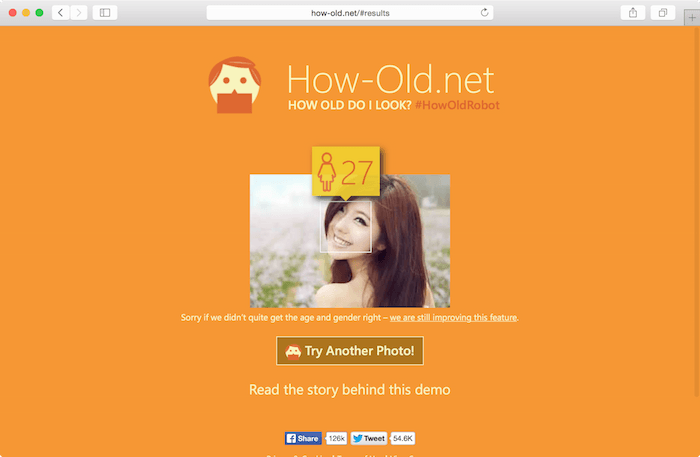
\includegraphics[width=0.5\linewidth]{how.png}
            \end{minipage}
  }
  \end{itemize}
\end{frame}

\section{方法論}

\subsection{模型輸入/輸出}
\begin{frame}{模型輸入/輸出}{Input/Output}
  \begin{itemize}
  \item {
    輸入為224*224的圖片
  }
 \item {
    輸出為1個代表Class的一維向量0到6 (0代表非人,1代表1代表 21~30,2代表31~40......以此類推)
  }
  \end{itemize}
\end{frame}
\subsection{模型的每一層}
\begin{frame}{模型的每一層}{Each layer of model}
  \begin{itemize}
  \item {
    卷積層1: 圖像通過6個5*5的filter做卷積
  }
 \item {
    池化層1: 圖像使用取2*2的filter將解析度降為1/4
  }
\item {
    卷基層2: 圖像通過16個5*5的filter做卷積
  }
\item {
    池化層2: 圖像使用取2*2的filter將解析度降為1/4
  }
\item {
    平坦層: 將圖像展開平攤
  }
\item {
    全連接層的隱藏層: 建128神經元,放棄一半的神經元
  }
\item {
    全連接層的隱藏層2:建84神經元,放棄一半的神經元
  }
\item {
    全連接層的輸出層: 建10神經元,輸出對應的數字
  }
  \end{itemize}
\end{frame}
\subsection{如何保存模型?}
\begin{frame}{如何保存模型?}{How you save model?}
  \begin{itemize}
  \item {
    使用network中的save函數儲存model成h5檔
  }
    \begin{minipage}[c][0.4\textheight][c]{\linewidth}
                \centering
                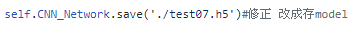
\includegraphics[width=1.0\linewidth]{save.png}
            \end{minipage}
  \end{itemize}
\end{frame}
\subsection{模型的大小}
\begin{frame}{模型的大小}{size of model}
  \begin{itemize}
  \item {
    61.9MB
  }
    \begin{minipage}[c][0.4\textheight][c]{\linewidth}
                \centering
                
\includegraphics[width=1.0\linewidth]{1561060727717.jpg}
            \end{minipage}
  \end{itemize}
\end{frame}
\subsection{你的損失功能是什麼?為什麼?}
\begin{frame}{你的損失功能是什麼?為什麼?}{What's your loss functions, and why? }
  \begin{itemize}
  \item {
     categorical crossentropy
  }
\item {
因為目標值為分類格式,我們有7個class,每筆都將會是7維向量,每個class只有表示該類的index為1,其餘為0
  }
  \end{itemize}
\end{frame}
\subsection{優化器和超參數設置}
\begin{frame}{優化器和超參數設置}{What's your optimizer and the setting of hyperparameter?}
  \begin{itemize}
  \item {
      Adam optimizer,lr=0.001(學習率)
  }
  \end{itemize}
\end{frame}
\section{數據集}
\subsection{數據集的大小}
\begin{frame}{數據集的大小}{The size of  dataset}
\begin{minipage}[c][0.4\textheight][c]{\linewidth}
                \centering
                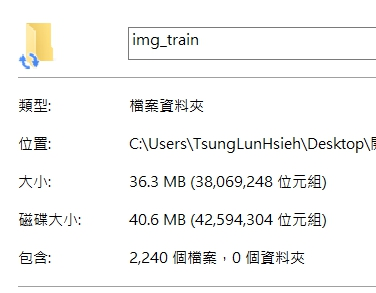
\includegraphics[width=0.5\linewidth]{1561052804594.jpg}
            \end{minipage}
\end{frame}
\subsection{如何收集/構建數據集?}
\begin{frame}{如何收集/構建數據集?}{How you collect/build your dataset?}
  \begin{itemize}
  \item {
    圖片來源:arge-scale CelebFaces Attributes (CelebA) Dataset
  }
  \item {
    由香港中文大學湯曉鷗教授實驗室公佈的大型人臉識別資料集。包含有200K張人臉圖片,人臉屬性有40多種
  }
 \item {
    從裡面20萬張的圖片挑選大約1000張左右的圖片使用,並且判斷年齡、自行撰寫CSV檔案
  }
 \item {
    有將圖片大小都調整為224*224,並且有部分資料有做4方向的翻轉
  }
  \end{itemize}
\end{frame}
\subsection{數據集中有多少個配對的樣本?}
\begin{frame}{數據集中有多少個配對的樣本}{How many paired samples in your dataset?}
  \begin{itemize}
  \item {
    訓練:1000筆
  }
  \item {
    驗證:1000筆
  }
 \item {
    測試:0筆
  }
  \end{itemize}
\end{frame}
\section{實驗評估}
\subsection{實驗環境}
\begin{frame}{實驗環境}{Experimental environment}
 \begin{itemize}
  \item {
    CPU: I5-6200U5 ; I7 6700HQ
  }
\item {
    Memory:8GB(DDR4X2)
  }
  \end{itemize}
\end{frame}
\subsection{您為訓練設置了多少個紀元?}
\begin{frame}{您為訓練設置了多少個紀元}{How many epochs you set for training?}
 \begin{itemize}
  \item {
    1000張的10代
  }
\item {
    3000張的2代
  }
  \end{itemize}
\end{frame}
\subsection{評估}
\begin{frame}{評估}{evaluation}
 \begin{itemize}
  \item {
    定性 - 圖片預測對錯
  }
\item {
    定量 - 準確率
  }
  \end{itemize}
\end{frame}
\subsection{現場演示}
\begin{frame}{現場演示}{Live demo}
  \begin{itemize}
  \item {
    現場演示
  }
  \end{itemize}
\end{frame}

\end{document}


